\documentclass{standalone}
\usepackage{tikz}
\usetikzlibrary{patterns}
\begin{document}
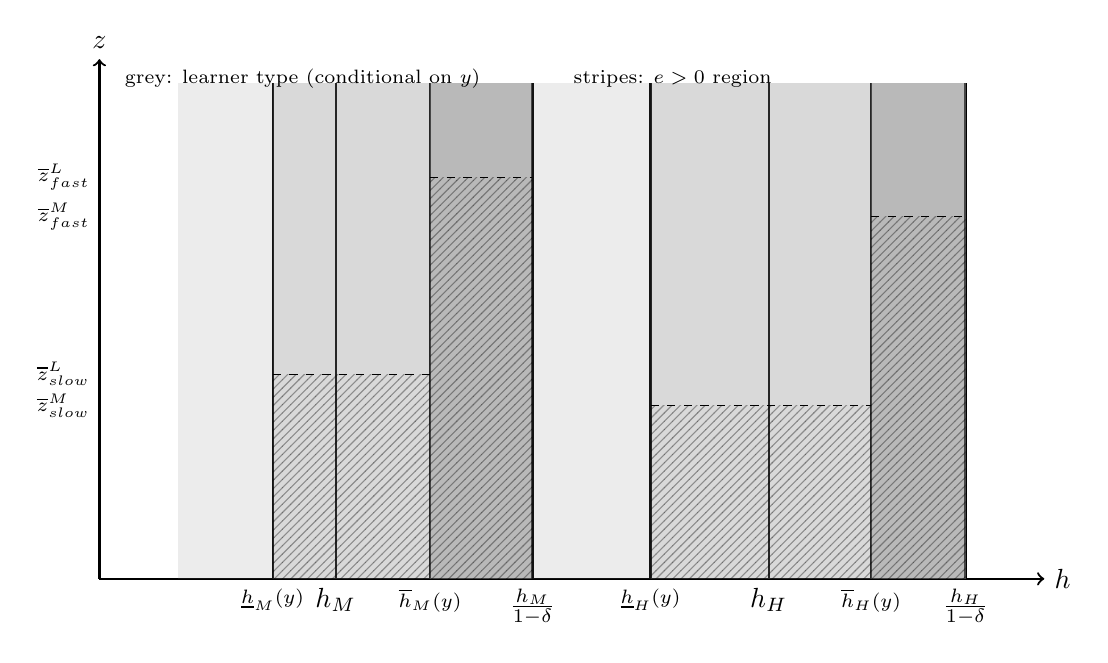
\begin{tikzpicture}

% Axes
\draw[thick,->] (-1,0) -- (11,0) node[right] {$h$};
\draw[thick,->] (-1,0) -- (-1,6.6) node[above] {$z$};

% Key h cutoffs
\draw[thick] (2,0) -- (2,6.3);
\node[below] at (2,0) {$h_M$};
\draw[thick] (4.5,0) -- (4.5,6.3);
\node[below] at (4.5,0) {$\frac{h_M}{1-\delta}$};
\draw[thick] (7.5,0) -- (7.5,6.3);
\node[below] at (7.5,0) {$h_H$};
\draw[thick] (10,0) -- (10,6.3);
\node[below] at (10,0) {$\frac{h_H}{1-\delta}$};

% h-cutoffs conditional on y (schematic placement, labels carry the economics)
% Relative to h_M
\draw[thick] (1.2,0) -- (1.2,6.3);
\draw[thick] (3.2,0) -- (3.2,6.3);
\node[below] at (1.2,0) {\scriptsize $\underline{h}_M(y)$};
\node[below] at (3.2,0) {\scriptsize $\overline{h}_M(y)$};
% Relative to h_H
\draw[thick] (6.0,0) -- (6.0,6.3);
\draw[thick] (8.8,0) -- (8.8,6.3);
\node[below] at (6.0,0) {\scriptsize $\underline{h}_H(y)$};
\node[below] at (8.8,0) {\scriptsize $\overline{h}_H(y)$};

% Grey shading: learner types (conditional on y), by h
% Left block (threshold h_M): [0,4.5]
\fill[gray, opacity=0.15] (0,0) rectangle (1.2,6.3);  % non-learners
\fill[gray, opacity=0.30] (1.2,0) rectangle (3.2,6.3); % slow learners
\fill[gray, opacity=0.55] (3.2,0) rectangle (4.5,6.3); % fast learners
% Right block (threshold h_H): [4.5,10]
\fill[gray, opacity=0.15] (4.5,0) rectangle (6.0,6.3);  % non-learners
\fill[gray, opacity=0.30] (6.0,0) rectangle (8.8,6.3);  % slow learners
\fill[gray, opacity=0.55] (8.8,0) rectangle (10,6.3);   % fast learners

% Stripes: region where e>0 (schematic, uses z cutoffs)
% Define schematic z cutoffs
\def\zSlowL{2.6}   % \overline{z}^L_{slow}
\def\zFastL{5.1}   % \overline{z}^L_{fast}
\def\zSlowM{2.2}   % \overline{z}^M_{slow}
\def\zFastM{4.6}   % \overline{z}^M_{fast}

% Left block: investment for slow learners (e_H) when z is low
\fill[pattern=north east lines, pattern color=black, opacity=0.35]
  (1.2,0) rectangle (3.2,\zSlowL);
% Left block: investment for fast learners (e_L) when z is below \overline{z}^L_{fast}
\fill[pattern=north east lines, pattern color=black, opacity=0.35]
  (3.2,0) rectangle (4.5,\zFastL);

% Right block: investment for slow learners (e_H) when z is low
\fill[pattern=north east lines, pattern color=black, opacity=0.35]
  (6.0,0) rectangle (8.8,\zSlowM);
% Right block: investment for fast learners (e_L) when z is low
\fill[pattern=north east lines, pattern color=black, opacity=0.35]
  (8.8,0) rectangle (10,\zFastM);

% Dashed horizontal cutoff lines (labels)
\draw[dashed] (1.2,\zSlowL) -- (3.2,\zSlowL);
\node[left] at (-1,\zSlowL) {\scriptsize $\overline{z}^L_{slow}$};
\draw[dashed] (3.2,\zFastL) -- (4.5,\zFastL);
\node[left] at (-1,\zFastL) {\scriptsize $\overline{z}^L_{fast}$};
\draw[dashed] (6.0,\zSlowM) -- (8.8,\zSlowM);
\node[left] at (-1,\zSlowM) {\scriptsize $\overline{z}^M_{slow}$};
\draw[dashed] (8.8,\zFastM) -- (10,\zFastM);
\node[left] at (-1,\zFastM) {\scriptsize $\overline{z}^M_{fast}$};

% Legend (minimal)
\node[anchor=west] at (-0.8,6.35) {\scriptsize grey: learner type (conditional on $y$)};
\node[anchor=west] at (4.9,6.35) {\scriptsize stripes: $e>0$ region};

\end{tikzpicture}
\end{document}

